\section*{Cíle laboratorního cvičení}
\begin{itemize}
  \item Seznámení se se signalizačním protokolem SIP.
  \item Peer-to-peer VoIP pomocí signalizace SIP.
  \item Komunikace VoIP pomocí signalizace SIP přes ústřednu.
\end{itemize}

\section*{Základní instrukce}
\begin{itemize}
  \item Připojte k počítači headset se sluchátky a mikrofonem.
  \item Přihlaste se do CentOS (F3), user/password {\tt user}/{\tt user4lab}.
  \item V pravé horní části obrazovky si {\bf zkontrolujte nastavení zvuku}. Sluchátka a mikrofon nastavte na optimální hlasitost.
  \item Otevřete si příkazovou řádku pro uživatele {\tt user}.
  \item Otevřete si příkazovou řádku pro uživatele {\tt root} (příkazem {\tt su}).
  \item V případě potřeby si otevřete další terminál v novém okně.
  \item Pracujte ve dvojicích, zkontrolujte, že máte počítač propojen
    přímým kabelem s přístupovým přepínačem (rozhraní enp2s0, zdířka E na patch panelu).
  \item Vyčistěte si pravidla ve firewall pomocí příkazu {\tt iptables --flush}.
\end{itemize}

\section{Peer-to-peer VoIP pomocí signalizace SIP}
V této části laboratoře nastavíte peer-to-peer VoIP komunikaci mezi počítači Vaší dvojice. a analizujete
Se svým sousedem nastavte komunikaci VoIP mezi Vašimi dvěma počítači bez použití ústředny (spojení peer-to-peer).

\begin{enumerate}
    \item V terminálu uživatele {\bf user} zapněte VoIP klienta Jitsi (pomocí {\tt jitsi \&}) a vyčkejte než se spustí okno programu.
    \item V menu {\bf Tools} $\rightarrow$ {\bf Options} $\rightarrow$ {\bf Accounts} přidejte nový účet. Pro ten nastavte pole {\bf Network} na možnost {\tt SIP} a následně {\bf SIP id} na Váš {\tt xlogin}.
    Vytvoření nového účtu potvrďte tlačítkem {\bf Add} a zkontrolujte, že se vytvořil {\it RegistrarLess SIP} účet (případně krok opakujte).
    \begin{figure}[h!]
    	\centering
    	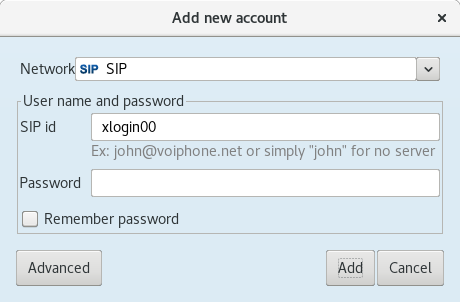
\includegraphics[scale=0.5]{img/account_p2p.png}
    	\caption{Informace o P2P SIP účtu.}
    	\label{fig:sip_account}
    \end{figure}
    \item V terminálu uživatele {\tt root} spusťte síťový analyzátor Wireshark (pomocí {\tt wireshark \&}) a začněte zachytávat pakety na rozhraní, kterým jste připojeni k síti ({\tt enp2s0}).
    \item Po spuštění zachytávání provozu na daném rozhraní nastavte display filtr tak, aby zobrazoval pouze protokol SIP.
    \item V hlavním okně programu zadejte do pole {\it Enter name or number} SIP adresu Vašeho souseda: \linebreak{\bf 10.10.10.1YY}, kde {\bf YY} je číslo počítače Vašeho souseda.
    \item Zavolejte Vašemu sousedovi stisknutím zeleného telefonu. Na druhém počítači přijměte hovor, vyzkoušejte, zda se se sousedem navzájem slyšíte a po chvíli hovor ukončete.
(V případě problémů se zvukem zkontrolujte, zda není v systému ztlumen mikrofon, či audio výstup, případně v aplikaci Jitsi v menu Tools $\rightarrow$ Options $\rightarrow$ Audio zkontrolujte nastavení zvukových zařízení.) 
    \item Proveďte analýzu navázaného spojení ve Wiresharku. Využijte podpory v menu {\bf Telephony $\rightarrow$ VoIP Calls}, kde uvidíte jednotlivé zaznamenané hovory. Vyberte příslušný hovor a pro zobrazení průběhu klikněte na volbu {\bf Flow}.
    \item Zakreslete spojení do grafu v protokolu. Uveďte, pomocí kterých protokolů a mezi jakými IP adresami a porty probíhá signalizace a přenos dat. Zjistěte použitý kodek pro přenos hlasu.
\end{enumerate}
Názvy a čísla podporovaných kodeků lze zobrazit v SIP/SDP zprávě v sekci {\bf Session Initiation Protocol} $\rightarrow$ {\bf Message body} $\rightarrow$ {\bf Session description protocol}:
\begin{figure}[h!]
  \centering
  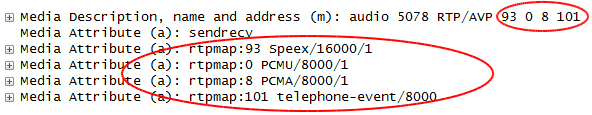
\includegraphics[scale=0.65]{img/3a.png}
\end{figure}

\noindent Informace o tom, který z podporovaných kodeků byl skutečně použit získáte z RTP paketů (Filter: RTP) podle čísla v poli {\bf Payload type}.
\begin{figure}[h!]
  \centering
  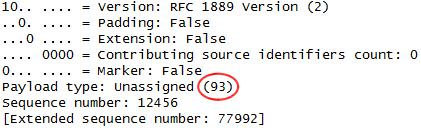
\includegraphics[scale=0.65]{img/3b.png}
\end{figure}


\section{Komunikace VoIP pomocí signalizace SIP přes ústřednu}
Se svým sousedem nastavte komunikaci VoIP mezi vašimi dvěma počítači pomocí SIP ústředny umístěné v laboratorní síti.

\subsection{Analýza registrace a odregistrace}
\begin{enumerate}
    \item Spusťte znovu zachytávání paketů v aplikaci Wireshark.
    \item Vraťte se do hlavního okna aplikace Jitsi a otevřite menu {\bf Tools} $\rightarrow$ {\bf Options} $\rightarrow$ {\bf Accounts}.
    \item Vytvořte nový účet\,--\,v poli {\bf Network} vyberte opět možnost {\tt SIP}, nasledně v poli {\bf SIP id} nastavte hodnotu {\tt user{\bf XX}@10.10.10.{\bf ZZZ}} a nakonec nastavte heslo na {\tt heslo{\bf XX}}, kde {\tt\bf XX} je vždy číslo Vašeho počítače a aktuální {\tt\bf ZZZ} adresu ústředny Vám sdělí cvičící.
     Obrázek \ref{fig:sip_account} ilustruje příklad korektního nastavení.
\begin{figure}[h!]
  \centering
  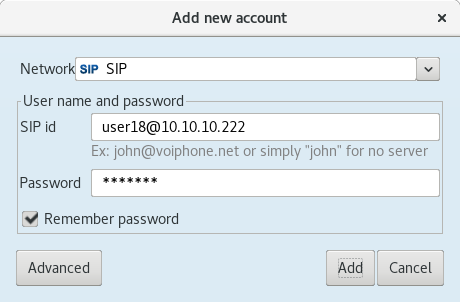
\includegraphics[scale=0.5]{img/account_asterisk.png}
  \caption{Informace o účtu ústředny.}
  \label{fig:sip_account}
\end{figure}
    \item Kliknutím na tlačítko {\bf Add} provedete registraci k ústředně.
    Pokud jste vše nastavili správně, mělo by se v pravém sloupci zobrazit {\bf SIP Online}. 
    {\it V případě neúspěchu v nastavení účet odeberte a znovu přidejte. Pokud ani toto nepomohlo, ukončete Jitsi a postupujte znovu od kroku 1, případně konzultujte problém se cvičícím.}
    \item V menu {\bf Tools} $\rightarrow$ {\bf Options} $\rightarrow$ {\bf Accounts} vytvořený SIP účet a klikněte na {\bf Delete}, čímž by měla proběhnout odregistrace od ústředny.
    \item Ve Wiresharku analyzujte registraci a odregistraci a zakresleslete jejich průběh do protokolu. Vyplňte požadované údaje a zjistěte, v čem se liší paket, kterým se registrujete, od paketu, kterým se odregistrujete.
\end{enumerate}


\subsection{Analýza hovoru přes ústřednu}
\begin{enumerate}
    \item Znovu se registrujte k ústředně stejně jako v předchozí sekci.
    \item Obnovte zachytávání paketů v aplikaci Wireshark.
    \item V hlavním okně programu Jitsi zadejte do pole pro telefonní číslo/adresu SIP adresu Vašeho souseda: {\tt 10{\bf YY}@10.10.10.{\bf ZZZ}}, kde {\bf YY} je opět číslo počítače Vašeho souseda a {\tt\bf ZZZ} aktuální adresa ústředny.
    \item Zavolejte Vašemu sousedovi a proveďte analýzu hovoru podobně jako u peer-to-peer hovoru.
    \item Zakreslete průběh spojení do grafu v protokolu.
    Zkombinujte informace z obou pracovních stanic a do protokolu zaneste úplnou komunikaci všech tří stanic.
    Uveďte, mezi kterými IP adresami a porty probíhá signalizace a mezi kterými přenos dat.
    Vyplňte, které protokoly se používají pro signalizaci a které pro přenos.
    Dále zjistěte, jaký kodek pro přenos hlasu byl použit.
\end{enumerate}

\section{Ukončení práce v laboratoři}
\begin{itemize}
  \item Počítač vypněte spuštěním (jako {\bf root}) skriptu {\tt /root/isa4/clean}.
\end{itemize}
